\documentclass{article}

% if you need to pass options to natbib, use, e.g.:
%     \PassOptionsToPackage{numbers, compress}{natbib}
% before loading neurips_2020

% ready for submission
% \usepackage{neurips_2020}

% to compile a preprint version, e.g., for submission to arXiv, add add the
% [preprint] option:
%     \usepackage[preprint]{neurips_2020}

% to compile a camera-ready version, add the [final] option, e.g.:
%     \usepackage[final]{neurips_2020}

% to avoid loading the natbib package, add option nonatbib:
     \usepackage[final, nonatbib]{neurips_2020}

\usepackage[utf8]{inputenc} % allow utf-8 input
\usepackage[T1]{fontenc}    % use 8-bit T1 fonts
\usepackage{hyperref}       % hyperlinks
\usepackage{url}            % simple URL typesetting
\usepackage{booktabs}       % professional-quality tables
\usepackage{amsfonts}       % blackboard math symbols
\usepackage{nicefrac}       % compact symbols for 1/2, etc.
\usepackage{microtype}      % microtypography
\usepackage{multirow}
\usepackage{makecell}
\usepackage{csquotes}
\usepackage{graphicx}

\title{Security and Privacy of Machine Learning - Homework 2}

\author{
  Wu-Jun Pei\\
  National Taiwan University\\
  \texttt{b06902029@ntu.edu.tw} \\
}

\begin{document}

\maketitle

\begin{abstract}
Despite the mightiness of deep nerual networks, several studies have shown that they are vulnerable
to adversarial examples,. In this homework, I built a
\end{abstract}

\section{Introduction}
In this homework, we're going to build a black-box defense on CIFAR-10 \cite{krizhevsky2009learning}
dataset.

\subsection{Threat Model}
As suggested in class \cite{spml0925}, we should state the considered threat model precisely. The
threat model I consider is listed as below:

\begin{itemize}
  \item The adversary has limited knowledge of the model, he only knows the model architecture, but
  is totally ignorant of the training process and the model weights.
  \item The adversary can perturb each pixel up to 8 (in 0-255 scale), which is given.
\end{itemize}

\section{Methods}
\subsection{Baseline Method}

\subsection{Adversarial Training}
Adversarial training \cite{madry2019deep}

\subsubsection{Adversarial Training}
Adversarial training may take a long time, and it's mostly contributed by \textit{generating
adversarial examples}.

\subsubsection{Adversarial Training on Ensemble Models}
Same as the previous subsection, adversarial training take a long time during the \textit{generating
adversarial examples} phase even in a single model setting. If we want to train an emsemble model of
several models, the time would grow significantly. For example, it only takes \textbf{TBD}. To
overcome the computational cost, I redesign the adversarial training process as:

\subsection{Preprocessing-based Defenses}
In my previous homework, I've already shown that some preprocessing-based defenses, such as vanilla
JPEG Compression, are effective enough to eliminate the influence of adversarial perturbations. In
this homework, I'm going to explore defenses that are more effective.

\subsubsection{Baseline}
Inspired by the preprocessing method TA used in the evaluation of previous homework, I setup the
baseline method as:

\begin{itemize}
  \item ColorJitter (brightness = 0.4, contrast = 0.4, saturation = 0.4, hue = 0.25)
  \item CenterCrop (size = 24)
  \item Pad (size = 4)
\end{itemize}

\subsubsection{Vanilla JPEG Compression}
We apply JPEG Compression on the entire image before feeding it to our model in order to reduce the
adversarial noise.

\subsubsection{SHIELD}
Similar to "Vanilla JPEG Compression", we divide the image into several equal sized subimages. For
each subimage, we apply different JPEG quality at random on it. And finally, we concatenate the
compressed subimages back.

\subsection{Evalution}
\label{section:evaluation}
To evaluate my work fairly, I unify the method to evaluate each model.

The adversarial examples are generated in the following way:
\begin{itemize}
  \item PGD attack, constrained to $l_2$ norm $\epsilon = 8 / 256$
  \item The number of iterations are 8, 16, 32, 64 and 128.
  \item The proxy models are \texttt{nin}, \texttt{resnet20}, \texttt{sepreresnet56},
  \texttt{densenet40-k12-bc}, and \texttt{diaresnet110}.
\end{itemize}

\section{Experiments and Findings}

\subsection{Adversarial Training}

\subsubsection{Adversarial Training Epochs}
\paragraph{Experiment Settings} In this experiment, we want to examine if increasing adversarial
training epochs improves the general adversarial accuracy. The model we used is \texttt{resnet20}
since it's more lightweight. We regenerate new adversarial examples every epoch, and each
adversarial example is generated with 8 iterations of PGD attack. We evaluate the model with
adversarial sets with different attack strengthes.

\paragraph{Findings} The experiment results are shown in figure \ref{img:exp-training-epochs}. We
can see that the model improves a lot in the first two epochs, and have no significant improvement
on evaluation set afterwards. Also, we can see that training on adversarial examples generated with
8 iterations have a fair performance on all other evaluation sets generated with larger iterations.
These findings suggest us that we can adversarially train our model with weaker adversarial set and
with less training epochs, saving computational costs. Although it seems robust to the evaluation
adversarial set, it's still vulnerable if the attacker knows the model weights. The accuracy on
newly generated adversarial examples are about 15\% on the last epoch.

\begin{figure}[ht]
  \begin{center}
  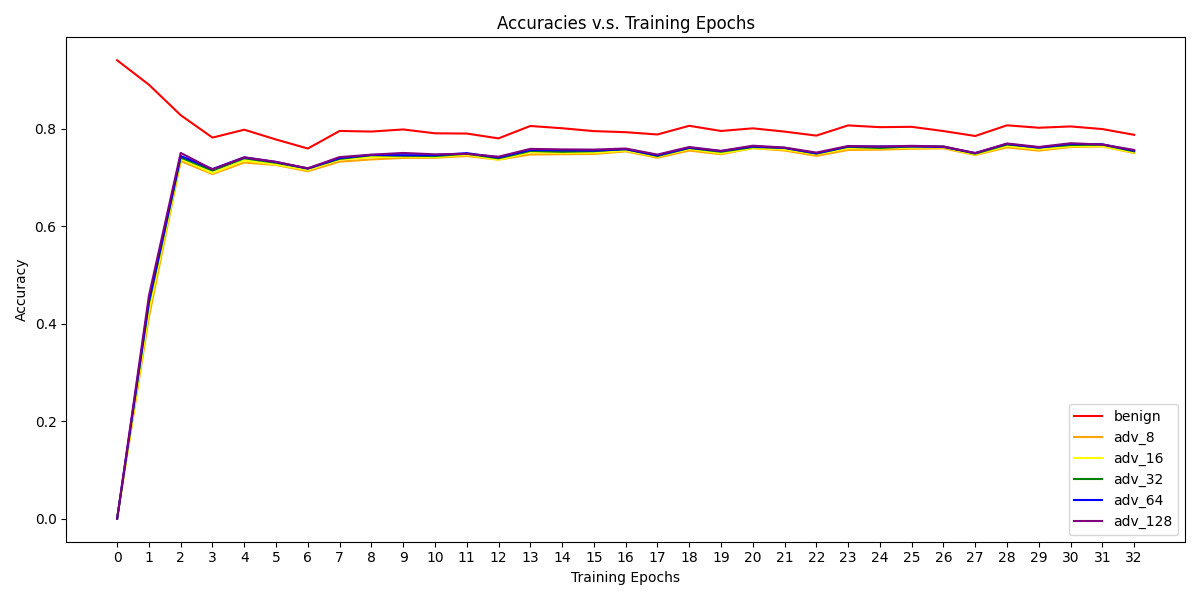
\includegraphics[width=0.8\linewidth]{imgs/exp-training-epochs.png}
  \end{center}
  \caption{\texttt{resnet20}'s accuracies on different training epoch, evaluated on adversarial sets
  generated with different number of iterations}
  \label{img:exp-training-epochs}
\end{figure}

\subsection{Preprocessing-based Defenses}
\paragraph{Experiment Settings} To test the effectivness of those defenses, I used two pretrained
\texttt{pytorchcv} models (without adversarial training), \texttt{resnet20} and \texttt{resnet1001}.
The adversarial examples are generated as described in section \ref{section:evaluation}
with 16 iterations of PGD.

\paragraph{Findings} The experiment results are shown in table
\ref{experiment:pgd-iterations}. We can see similar performance on the two models. The
baseline method has little effect on adversarial examples, while both vanilla JPEG compression and
SHIELD are more effective. To take a closer glimpse, we can see that vanilla JPEG compression method
has better on both benign set and adversarial set. I guess that it may result from that the image
size in CIFAR-10 is already small (32x32), and the smaller splitted images will not benefit from the
JPEG compression.

\begin{table}
  \label{experiment:pgd-iterations}
  \centering
  \caption{Evaluation of different preprocessing based defense. The plus sign (+) indicates the
    benign set while the minus sign (-) indicates the adversarial set.}
  \begin{tabular}{ccccccccc}
    \toprule
    & \multicolumn{4}{c}{resnet20} & \multicolumn{4}{c}{resnet1001} \\
    \cmidrule(r){2-5} \cmidrule(r){6-9}
    Defense Method            & Train + & Train - & Val. +  & Val. -  & Train + & Train - & Val. +  & Val. -  \\
    \midrule
    None                      & 0.9865  & 0.0000  & 0.9403  & 0.0001  & 1.0000  & 0.3962  & 0.9672  & 0.3420  \\
    Baseline                  & 0.8622  & 0.1957  & 0.8181  & 0.1950  & 0.9403  & 0.4847  & 0.8792  & 0.4462  \\
    JPEG (quality = 60)       & 0.8211  & 0.6389  & 0.7924  & 0.6162  & 0.9257  & 0.8239  & 0.8671  & 0.7563  \\
    SHIELD (block size = 4)   & 0.7917  & 0.5902  & 0.7634  & 0.5688  & 0.8939  & 0.7719  & 0.8322  & 0.7068  \\
    \bottomrule
  \end{tabular}
\end{table}


\section{Final Decision}
The final model I use is

\begin{itemize}
  \item An ensemble model consisting of ....
  \item Adversarial training for epochs, adversarial examples are regenerated for x iterations every
  y epochs.
  \item Equipped with a single preprocessing-based defense, JPEG-Compression with quality 60.
\end{itemize}

\section{Conclusion}

\bibliographystyle{ieeetr}
\bibliography{citation}

\end{document}
